\section{Education and outreach efforts}
Having developed a portable prototype of the apparatus, investigations into its use as an educational tool were started. The aims of this part of the project were to identify the ability range of students who could benefit from such outreach, to develop and implement an outreach lesson, and assess its effectiveness in engaging students in undergraduate physics.

Considering the relatively high level of understanding of quantum physics required to grasp both the theory behind our experiment and its implications, sixth-form students were selected as the primary target group. To that end, teachers at schools project members had attended were contacted, and a school in Chesham selected for an outreach lesson. A lesson plan (Section \ref{lessonplan})) was developed, with significant feedback from Dr. Mark Fuller, outreach officer for the department. This, alongside a Powerpoint (Appendix \ref{app:powerpoint}), was delivered on the 7th March.

Evaluation of the lesson was conducted through a paper survey, overleaf, and through feedback from the class teacher. Students used a four point rate their agreement with various statements corresponding to our outreach aims. Each statement was then assigned an "agreement score", defined as $\frac{\sum{x}}{4N}$, where x is the score given to each statement and N is the number of students in the class. The results of this are shown in Figure \ref{fig:evaluationchart}.

\begin{figure}[h]
\centering
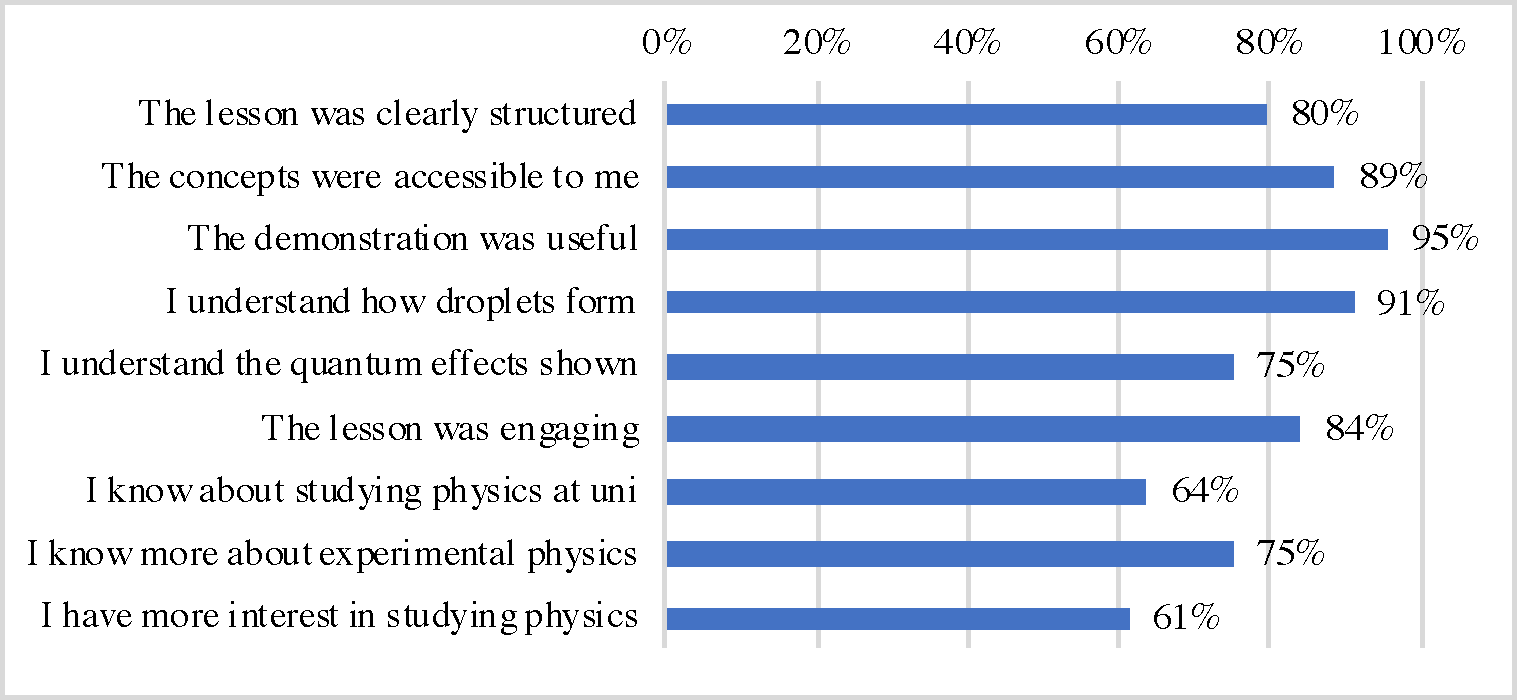
\includegraphics[width=\textwidth]{education/evaluationchart.pdf}
\caption{Percentage agreement with evaluation statements. Note that the final statement included a "not applicable" option, so has a smaller sample size.}
\label{fig:evaluationchart}
\end{figure}

This evaluation showed that students generally found the lesson enjoyable and engaging, and valued the use of the prototype as a demonstration aid. Understanding of the quantum effects shown by our experiment was less robust, although this could be due to the year 12 students being unfamiliar with such topics beforehand, as they don't study quantum physics in detail until year 13. Most lacking from this intervention was an understanding of the experience of studying physics at university. It would be relatively easy to devote more time to this in future sessions, depending on the precise aims of the workshop, which should provide sufficient improvement.

\clearpage

\subsection{Lesson Plan} \label{lessonplan}

\noindent Date: 7/3/18

\noindent Lesson: Physics

\noindent Year: 12/13

\noindent Levels: Any

\noindent Tutor: Group 13

\noindent Topic: Quantum mechanical effects using bouncing droplets


\noindent Learning objective and outcomes:
\begin{enumerate}
\item How droplets can bounce on a vibrating surface
\item What quantum mechanics is, and what effects we can observe some of these things from the apparatus
\item Have an insight into undergraduate physics and some of the hands on work it can entail
\end{enumerate}

\noindent \textbf{Introduction} (5 mins): Introduce ourselves and the reasons we're there for. 

\noindent \textbf{Starter} (10 mins): Start discussion into what quantum physics is. To facilitate audience participation, ask students to discuss amongst themselves for 3 minutes and propose ideas. Then ask for these ideas, and add/correct responses as required

\noindent \textbf{Mini-lecture} (10 mins): How do droplets form? (Diagram on board) Explain that (but not how) these droplets demonstrate QM behaviour. Starting from basic diagrams and maybe a recording of bouncing droplet motion, explain how droplets bounce. Then explain that these droplets replicate quantum behaviour. Attempt to limit the scope of this behaviour by mentioning specific effects. Don't explain how this link occurs yet.

\noindent \textbf{Demonstration} (10 mins): Explain apparatus and highlight important components. Execute a run through of the apparatus (need to find a way to get a live feed to projector). Specifically demonstrate bouncing droplets, walking droplets and multiple droplet motion. Take time to allow for students to run through experiment themselves, e.g. by making droplets and playing with the frequencies/bass. As there is only one apparatus, take suggestions from students. 

\noindent \textbf{Discussion} (10 mins): Discuss in groups how these droplets display behaviour. Ask students to also note down any interesting behaviours they observe. May have to use lab based recordings/ simulation for double slit diffraction or other interesting effects we want to mention

\noindent \textbf{Plenary} (10 mins): Assert that droplets demonstrate XYZ behaviour, make limitations clear. Wrap up by emphasising learning objectives, link to Veritasium for more details. It would be quite useful to part on an entertaining note. See if music/ colourful lights can make the apparatus do something more exciting. 

\noindent \textbf{End of session} (10 mins): 10' Q&A on Physics at Uni, completion of end of session assessments. 



\noindent \textbf{Key words}: Pilot wave theory, guiding wave equation, wave particle duality, Destructive and constructive interference

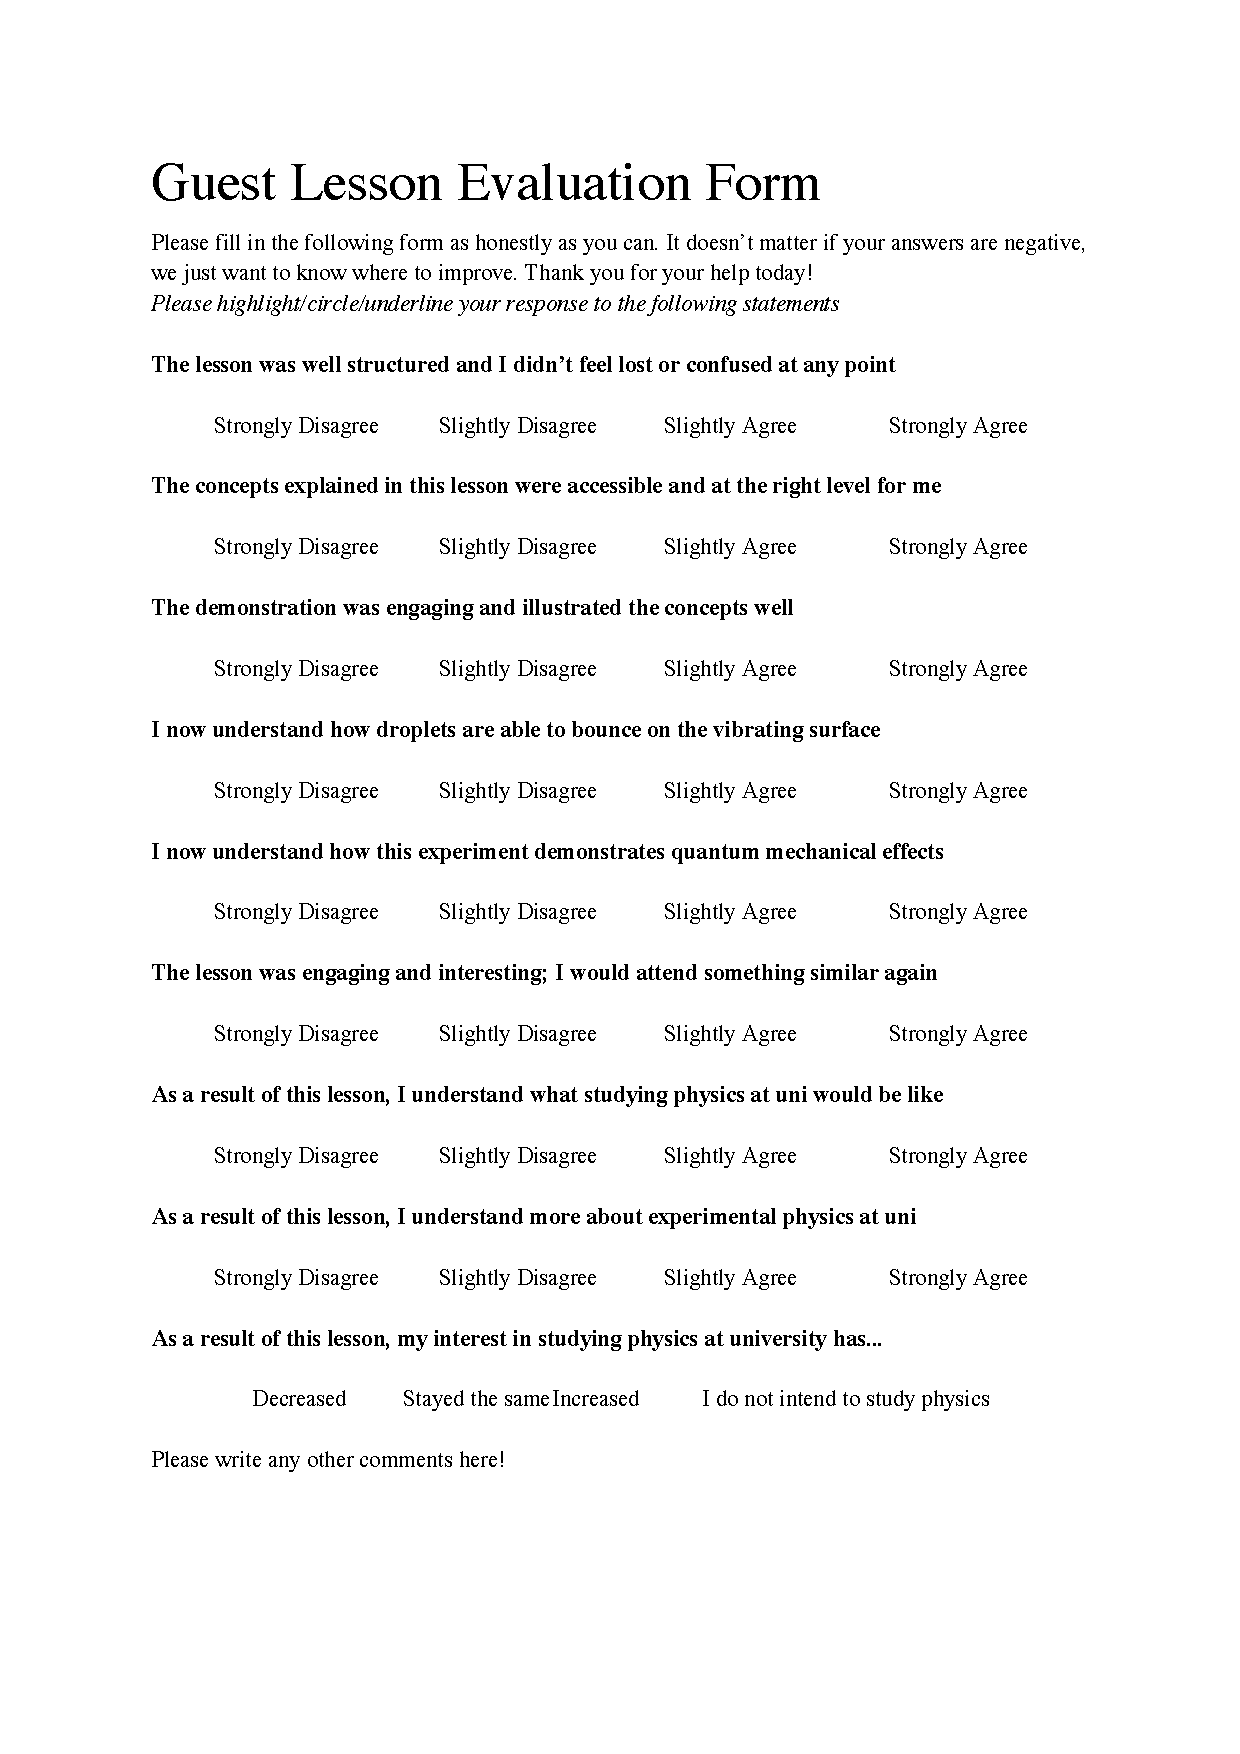
\includepdf{education/evaluation.pdf}